%        File: main.tex
%     Created: Tue Dec 10 09:00 PM 2013 E
% Last Change: Tue Dec 10 09:00 PM 2013 E
%     Handy hints for vim-latex-suite: http://vim-latex.sourceforge.net/documentation/latex-suite/auc-tex-mappings.html
%     Character list for math: http://www.artofproblemsolving.com/Wiki/index.php/LaTeX:Symbols
%
\documentclass[a4paper]{article}

\usepackage[pdftex,pagebackref,letterpaper=true,colorlinks=true,pdfpagemode=none
,urlcolor=blue,linkcolor=blue,citecolor=blue,pdfstartview=FitH]{hyperref}

\usepackage{amsmath,amsfonts}
\usepackage{graphicx}
\usepackage{color}
\usepackage{natbib}
\usepackage{hyperref}
\setlength{\oddsidemargin}{0pt}
\setlength{\evensidemargin}{0pt}
\setlength{\textwidth}{6.0in}
\setlength{\topmargin}{0in}
\setlength{\textheight}{8.5in}

\setlength{\parindent}{0in}
\setlength{\parskip}{5px}

\begin{document}
\textbf{Projection Methods for Viscoplasticity -- T. Ben Thompson}
\tableofcontents

\section{Introduction}
In the lower crust and upper mantle, a significant component of deformation occurs by slow viscous creep. 
After an earthquake, the stresses are increased and the rate of viscous creep accelerates \citep{Burgmann2008}.
I am interested in solving for the creep velocities and stress evolution in the lower crust and upper mantle after an earthquake.
Ultimately, I would like to include temperature evolution and the coupling between temperature and creep rates. 

One of the critical assumptions of slow creep flow is that inertia is negligible. Ignoring elasticity, the problem reduces
to a Stokes' flow. Mathematically, solving a Stokes flow requires solving Poisson's equation, a relatively simple endeavor. 
However, in the presence of elasticity (a viscoelastic material), the problem becomes more complex. 
If the viscosity is rate- or state-dependent (a viscoplastic material), the problem is nonlinear and even more difficult.
I demonstrate a method to reduce a viscoplastic problem in the limit of short time to the solution of an ODE and a Poisson equation.
The approximation is implemented in a numerical code.
The method is based on an analogy with the popular projection method for solving the Navier-Stokes equations \citep{Guermond2006}
In the future, the method I develop could be extended to consider thermomechanical coupling in the crust.

\section{Problem}
For a viscoelastic maxwell model, the constitutive relation can be written:
\begin{equation}
    \dot\epsilon = \frac{1}{2\eta}\sigma + \frac{1}{2\mu}\dot\sigma
    \label{const}
\end{equation}
where $\dot\epsilon$ is the strain rate, $\eta$ is the viscosity, $\mu$ is the shear modulus, and $\sigma$ is the stress. 

Ignoring inertia, momentum conservation gives
\begin{equation}
    \nabla \cdot \sigma = \rho \dot v = 0
    \label{mom}
\end{equation}

I am interested in solving these equations in the aftermath of a large upper crustal earthquake. 
A common description of the domain for this problem is shown in Figure 1. 
\begin{figure}[h!]
  \caption{A common model for the viscoelastic relaxation of the crust and upper mantle after a strike slip earthquake.}
  \centering
    \includegraphics[width=3.5in,height=3.0in]{twolayer.png}
\end{figure}

The earth's surface is treated as traction free.
The upper layer of the crust is treated as purely elastic and lies over a viscoelastic half space.
The initial conditions result from a screw dislocation with constant offset in the out-of-plane direction \citep{Segall2010a}.

In the geometry in Figure 1, the problem can be analytically solved assuming constant viscosity using Laplace transforms.
In an antiplane shear geometry, the Laplace transform of equation \ref{const} is:
\begin{equation}
    \bar\epsilon = \frac{\mu^{-1} s + \eta^{-1}}{2s}\sigma
    \label{laplace}
\end{equation}
where $s$ is the Laplace domain frequency variable. 
This is exactly equivalent to an elastic problem where the coefficient of $\sigma$ is the elastic modulus. 
So, solving the constant viscosity viscoelastic problem reduces to inverting the Laplace transform of an elasticity
problem\citep{Nur1974}. This is known as the correspondence principle. 

I plan to develop an efficient approximation to the solution of these viscoelastic equations in the limit of short time. The
method will be able to handle arbitrary viscosity functions, as well as spatial variation in the elastic moduli. 
\section{An Analogy}
In fluid dynamics, the projection method is a common technique for numerically solving the Navier-Stokes equations. 
The projection method can be thought of as a predictor-corrector type method or as a numerical analog of dominant balance \citep{Guermond2006}.
The prediction steps proceeds by approximating the pressure gradient term, $\nabla p$, as an extrapolation of the 
pressure from previous time steps. 
Hence, the prediction step can be thought of as a advection-diffusion equation with a source term. 
In non-dimensional form:
\begin{equation}
    \frac{\partial u}{\partial t} + (u \cdot \nabla)u ~= ~ -\nabla p^* + \frac{1}{Re}\nabla^2u
    \label{ns_pred}
\end{equation}
where $u$ is the fluid velocity and $p^*$ is the extrapolated pressure (given). Call the solution to this equation $\bar u^{n+1}$.

Because the predictor step ignores pressure evolution, the velocity continuity equation,
\begin{equation}
    \nabla \cdot u = 0
    \label{continuity}
\end{equation}
will be violated. 
The job of the corrector step is to fix this continuity violation.
The predictor step can be thought of as a dominant balance of the original Navier-Stokes equations where I ignore the pressure evolution.
In the corrector step, I take the complementary dominant balance, ignoring all terms except for the pressure evolution. This ensures
that I never ``double count'' a term. The equation is:
\begin{equation}
    \frac{\partial u}{\partial t} = -\nabla p
\end{equation}
paired with the continuity constraint, equation \ref{continuity}.
The important step is to discretize the time derivative:
\begin{equation}
    \frac{u^{n+1} - \bar u^{n+1}}{\Delta t} = -\nabla p
    \label{discrete_corrector}
\end{equation}
Then, because I would like to enforce the continuity constraint,
I take the divergence of both sides, which simplifies because the divergence of the solution is 0.
\begin{equation}
    -\frac{\nabla \cdot u^{n+1} - \nabla \cdot \bar u^{n+1}}{\Delta t} = -\frac{\nabla \cdot \bar u^{n+1}}{\Delta t} = \nabla^2 p
    \label{poisson_pressure}
\end{equation}
This is a Poisson equation for the pressure, because the term on the left-hand side has already been computed.
Once the Poisson equation is solved, the velocity can be updated using Equation \ref{discrete_corrector} and another time step begins. 
This Poisson equation can also be derived by taking the solution from the corrector step and asking what is the closest vector on the
surface $\nabla \cdot u = 0$. This step of projecting onto a divergence-free solution surface is why the technique is known as the projection method.

The pressure from the previous time step is a reasonable approximation for the pressure during the current time step.
So, the solution derived by the predictor step is a reasonable guess for the velocity. The corrector step simply ensures that
the final velocity represents an incompressible fluid. These statements can be quantified to show that the
predictor-corrector splitting has error $O(\Delta t)$ \citep{Rannacher1992}

In the viscoelastic problem, I will decompose the problem into a predictor-corrector form in a similar way. 
\section{Projection Method for Viscoelasticity}
To simplify the discussion, I will only consider antiplane strain problems. I do not think that I ever rely on this fact, hence generalizing what I describe 
to plane strain or three dimensions should be straightforward. 
In an antiplane geometry, $\frac{\nabla v}{2} = \dot \epsilon$, so I will proceed considering the scalar velocity rather than the
strain rate and a vector stress $(\sigma_{xz}, \sigma_{yz}, 0)$.

In the viscoelastic case, I treat the stress as analogous to the Navier-Stokes velocity because it is the divergence-free variable. 
The velocity is then analogous to the pressure in the Navier-Stokes equations. So, the predictor step is:
\begin{equation}
    \nabla v^{*} = \frac{1}{\eta}\sigma + \frac{1}{\mu}\dot\sigma
\end{equation}
where $v^{*}$ is the extrapolated velocity and is considered given. Hence, this equation is an ordinary differential equation for $\sigma$.
Call the solution at time $t = \Delta t$, $\bar\sigma^{n+1}$.
The corrector step is the complementary dominant balance:
\begin{equation}
    \nabla v = \frac{1}{\mu}\dot\sigma
    \label{corrector}
\end{equation}
Discretizing and taking the divergence gives:
\begin{equation}
    \nabla^2 v = \frac{1}{\Delta t \mu}\bar\sigma^{n+1}
\end{equation}
because $\nabla \cdot \sigma^{n+1} = 0$.
This is a Poisson equation for the velocity. The solution is input to Equation \ref{corrector} to update the stress. Then, another time step begins.

The computational efficiency of this splitting is significant. 
The main nonlinearity of interest is in the viscosity $\eta$, but this nonlinearity only appears in the ODE predictor step. There is a wealth
of very powerful techniques to solve ODEs and any of them can be applied to the predictor step. The corrector step consists of a \textit{linear} Poisson equation.
This is another readily solved problem and, if all the inputs are smooth, can be solved extremely quickly using fast fourier transform methods.
Hence, a difficult nonlinear PDE equation with a divergence-free constraint has been decomposed to a pair of easily solved differential equations. 
Although the theoretical $O(\Delta t)$ error analysis performed for the Navier-Stokes projection method does not apply for this scenario, it seems reasonable
to expect a similar order of convergence. 


\begin{figure}[h!]
  \caption{The numerical solution is computed on the staggered grid shown here, so that unphysical velocity oscillations do not form.}
  \centering
    \includegraphics[width=1.0\textwidth]{staggered_grid.png}
\end{figure}
\section{Numerical Example}
The problem is solved on a staggered grid shown in Figure 2. On a naively implemented collocated grid, centered finite difference
approximations to the gradient and the divergence skip over the middle node
\begin{equation}
    \frac{\partial u_i^n}{\partial x} = \frac{u_{i+1}^n - u_{i-1}^n}{2\Delta x}
\end{equation}
resulting in the possibility of numerically acceptable checkerboard solutions, a physically unacceptable result. An analogous problem
is observed for the Navier-Stokes projection method. More complex methods have been developed to remedy the problem on a collocated grid.

Comparing the numerical solution with an analytical solution is possible, but requires care. In Figure 3, 4 and 5, the results of the numerical projection method are shown. Figure 5 compares the results with an analytical solution at the surface. All plots are displayed 100 years after the screw dislocation offset with a
viscosity $\eta = 5 \times 10 ^ 19 \textrm{Pa s}$.
The analytical solution represents the viscoelastic relaxation of maxwell viscoelastic half-space beneath an elastic surface layer after a screw dislocation
with magnitude $\Delta u$ in meters.
\begin{equation}
    v(x, t) = \frac{\Delta u}{\pi t_R} e ^{-t/t_r} \sum_{n=1}^{\infty} \frac{(t/t_R)^{n-1}}{(n-1)!} \tan^{-1}\left(\frac{2xd}{x^2 + (2nH)^2 - D^2}\right)
    \label{analytical}
\end{equation}
where $H$ is the thickness of the elastic layer, $D$ is the depth to which the fault penetrates, and $t_R = \frac{2\eta}{\mu}$ is the maxwell relaxation
time scale. The solution can be derived using the viscoelastic Laplace domain correspondence principle. The corresponding elastic solution is derived as 
the superposition of an infinite series of images that maintain traction continuity at the bottom of the elastic layer and the traction free surface condition.

Because the numerical solution must use a finite domain, there will be significant differences between the analytical and numerical solutions solve different problems.
Because of the elliptic character of the PDE, the difference in boundary conditions will influence the entire solution, so I cannot resort
to comparing the solutions far from the boundary.
Despite this, the qualitative character of the solutions should be similar and the quantitative difference should be much less than 100\%. 

Figures 3 demonstrates the expected qualitative behavior of the velocity field. Figure 4 shows the expected behavior of the time evolution of
surface velocities. 

As shown in the plot of surface velocities in Figure 5, the difference between the analytical solution
and the numerical projection method solution is on the order of 10\%, which should be considered a success given the
difference in boundary conditions.

\begin{figure}[h!]
  \caption{The velocity field 100 years after a 2 meter screw dislocation.}
  \centering
    \includegraphics[width=1.0\textwidth]{velocity_2D.png}
\end{figure}

\begin{figure}[h!]
  \caption{Evolution of surface velocity over time. Shows the velocity after 25, 50, 75, and 100 years.}
  \centering
    \includegraphics[width=1.0\textwidth]{velocity_over_time.png}
\end{figure}

\begin{figure}[h!]
  \caption{A comparison of the surface velocity 100 years after a 2 meter screw dislocation showing both the viscoelastic two layer solution and the numerical projection method solution.}
  \centering
    \includegraphics[width=1.0\textwidth]{velocity_comparison.png}
\end{figure}
\clearpage
\section{Discussion}
Although I have not developed any theoretical results regarding the numerical stability of the scheme demonstrated here, numerical tests do not demonstrate any 
instability even for unreasonably large time steps. Thus, this projection method may be superior to the similar method described by \citet{Zienkiewicz1974},
where the time step is restricted to undesirably small values by a stability criterion.
\citet{Hughes1978} prove unconditional stability for a finite element scheme for viscoplasticity. However, in their scheme the nonlinearity in the 
viscosity remains in the matrix inversion step so that Newton iterations must be performed. Thus, their scheme is significantly less efficient than the
one presented here. Furthermore, the methods presented by \citet{Hughes1978}, \citet{Zienkiewicz1974}, and \citet{Melosh1980} are limited to a 
finite element formulation, whereas the Poisson equation in the method described here could be solved any of a variety of methods. Chebyshev pseudospectral
methods would give excellent convergence and order of magnitude computation time decreases (\citep{Trefethen2000}). 

Much more verification will be required to determine if the results described hold up in more difficult problems.
One step could be to use the method of manufactured solutions to test the numerical method with a more appropriate analytical problem.
Convergence tests would also demonstrate the method's accuracy. 

The method I implemented is very simple translation of original projection method described by \citet{Chorin1968}. 
Variations on the method have been developed since that improve the error from first to second order in time. I think it
is likely that these variations will have a direct analog in viscoelasticity.

The code is available on \textbf{github} at \url{https://github.com/tbenthompson/viscosaur/tree/master/source/projection}. 
The code repository is being actively developed, so to obtain the exact code used here, checkout revision code ``74749c1cbc7d2dce71a5bfd2273a40e866132a61''. 
Exceution begins in the ``ProjController'' class.
\bibliographystyle{agufull08}
\bibliography{/home/tbent/projects/library.bib}
\end{document}


